% Chapter for background.

\chapter{Background}
\label{ch:background}

In this section we will discuss essential background information to this project.
First we discuss the specific terminology used in this paper. Next we discuss
previous work done that relates to this project.

\section{Technical Background}

As already mentioned, this project aims to produces a new teaching tool for
6.01. As such, let us first discuss the scope of circuits in 6.01.

\subsection{What are our circuit components?}

The rudimentary circuit components that students work with are resistors,
operational amplifiers (op-amps), and potentiometers (pots). Students start out
by building very simple circuits, and then go on to building
more complicated circuits with time. The simplest circuits that students build
aim to control lego motors in a particular way. In constructing these circuits,
students use $6$-pin \textit{motor connectors} to connect their circuits to
lego motors.
The more complicated circuits students build interact with robots that were
built specifically for the purposes of 6.01. One of the 6.01 robots is displayed
in Figure \ref{fig:robot}. Students use $8$-pin \textit{robot connectors} to
connect their circuits to robots. The robots can be equipped with heads that have
vision capabilities. Each head has a rod attached to a potentiometer. Also attached
to the rod are a lego motor and a plate containing two photosensors positioned
at a $90\,^{\circ}$ angle from each other. The
photosensors are used to serve as eyes for the robot. This setup allows us to
turn the head by controlling the motor and inquire the current position of the
head by probing the pot. Figure \ref{fig:robot} displays a robot with a head.
Students use $8$-pin \textit{head connectors} to connect their circuits to
robot heads.

All together, our components are resistors, op-amps, pots, motor connectors,
robot connectors, and head connectors.

\begin{figure}
\begin{center}
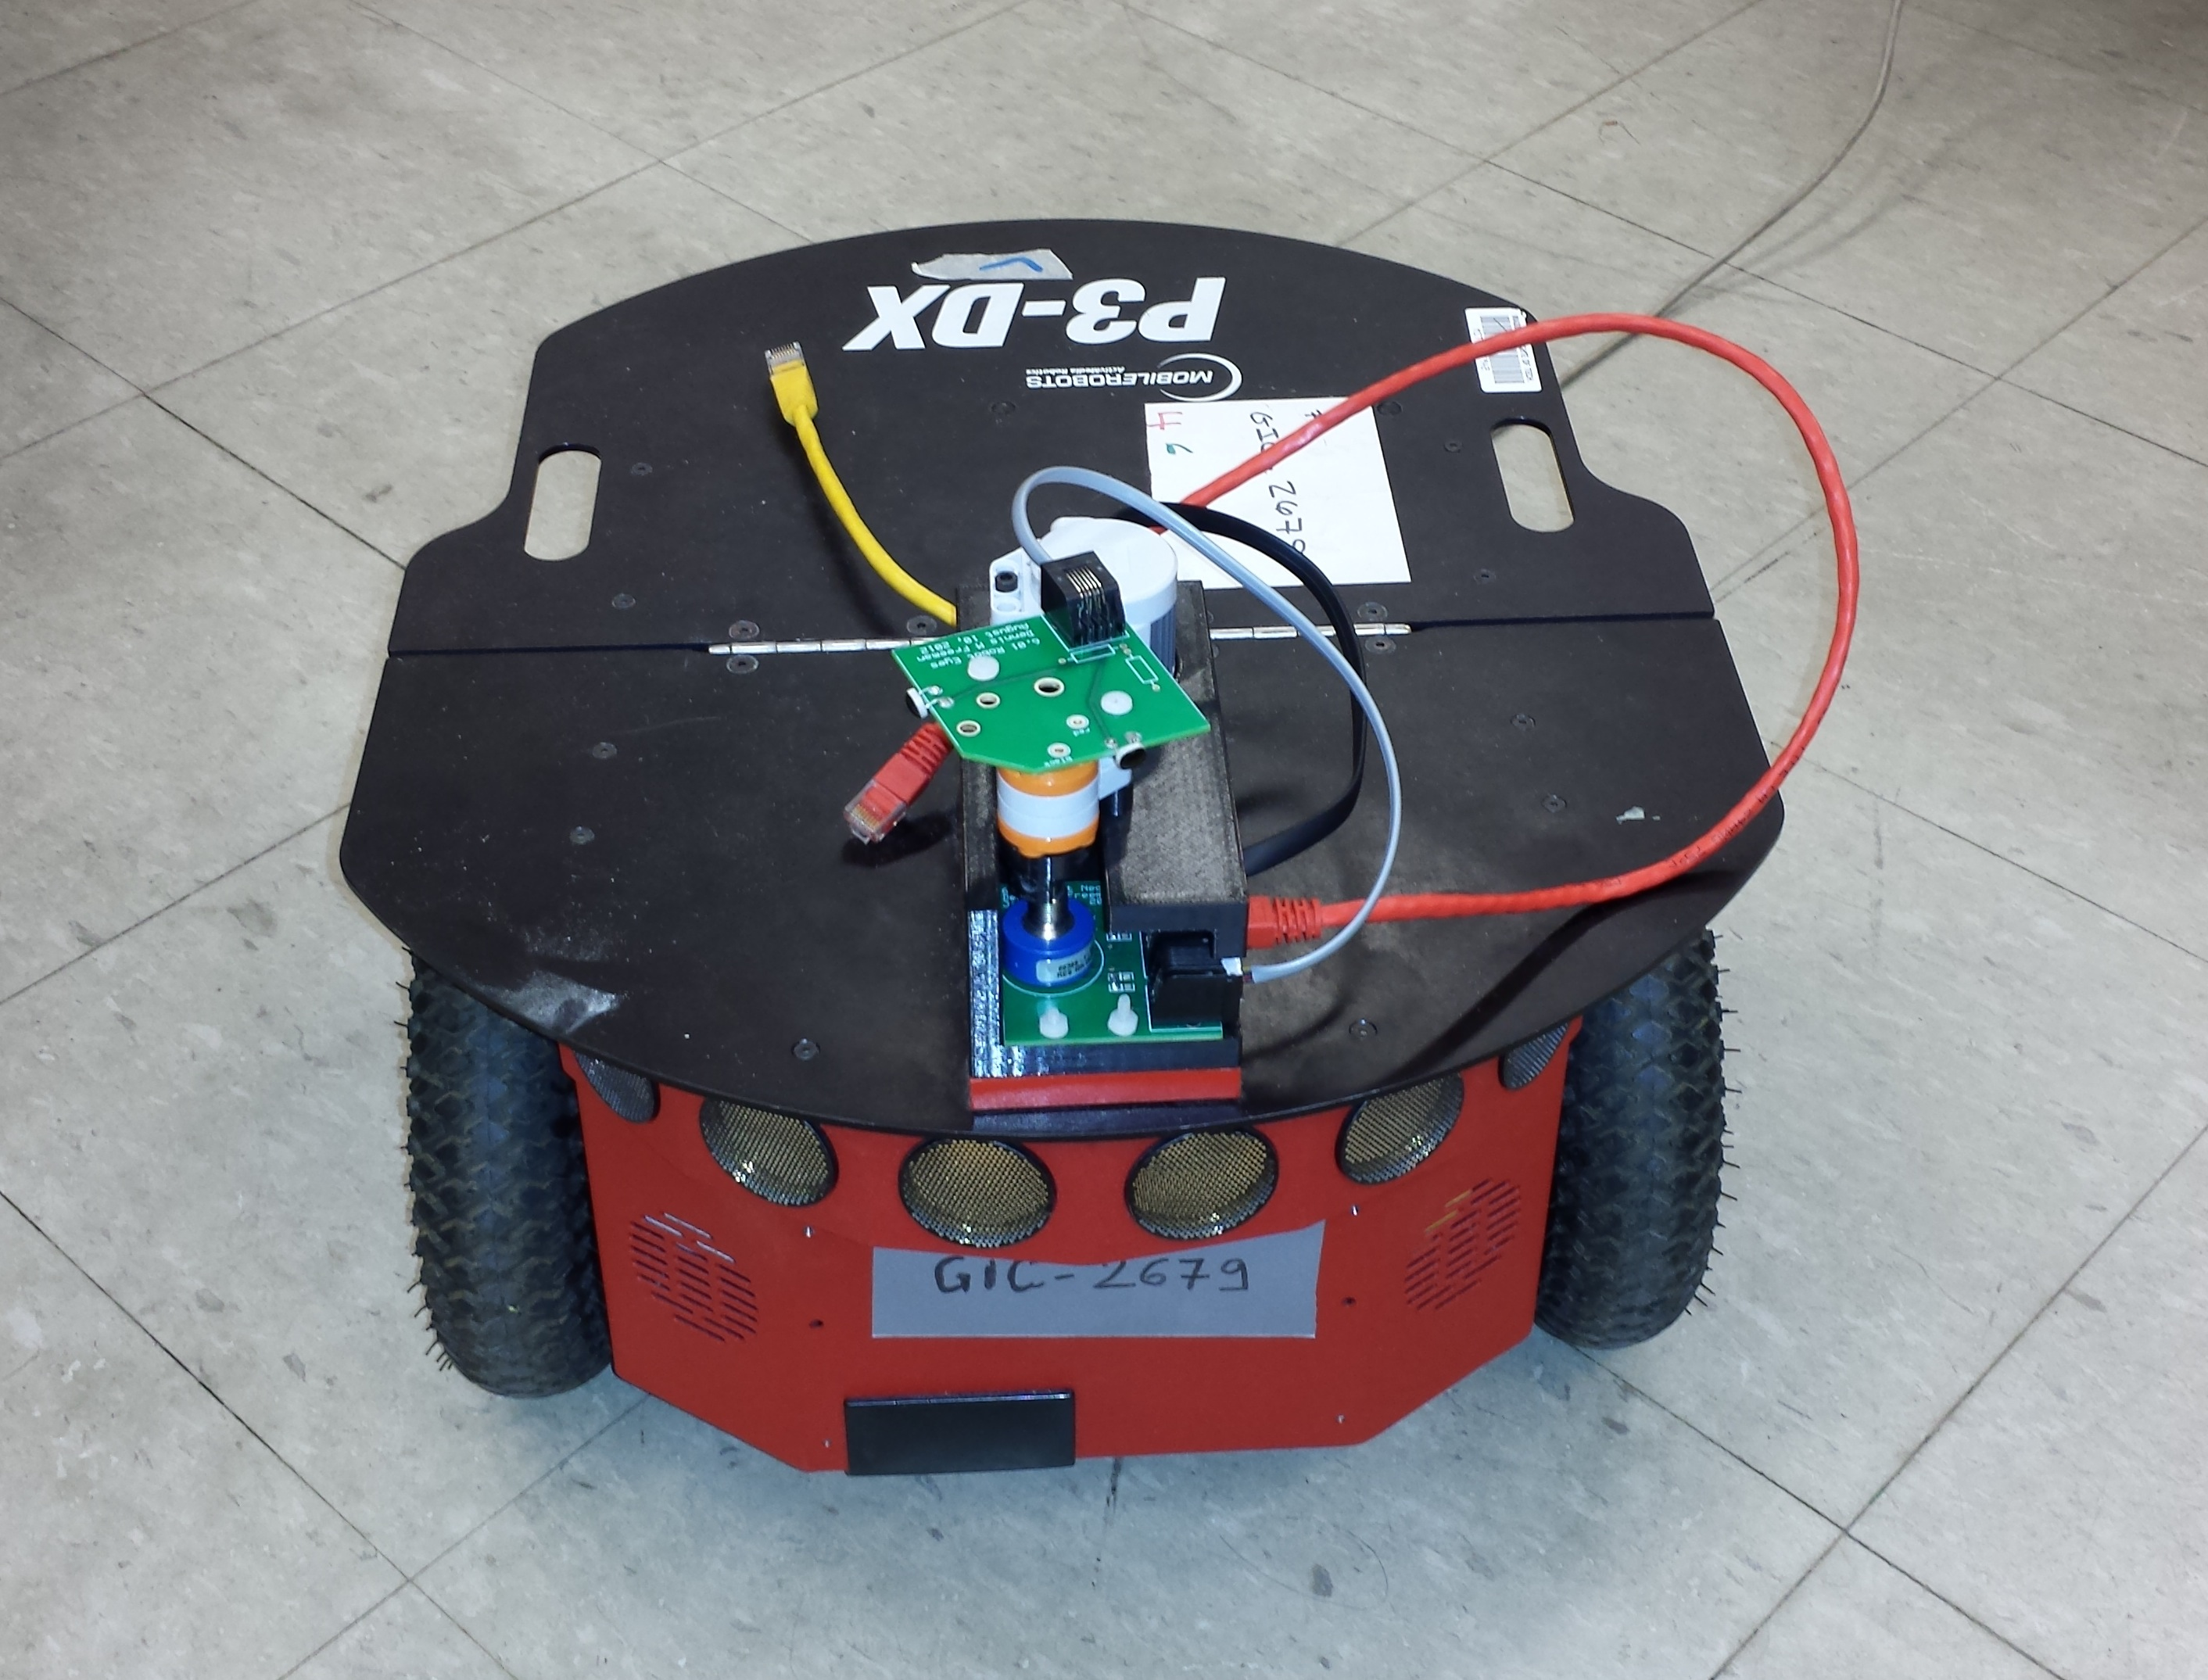
\includegraphics[width=\textwidth]{Images/robot.jpeg}
\caption{6.01 robot.}
\label{fig:robot}
\end{center}
\end{figure}

\subsection{What is a circuit schematic?}

Throughout this paper, the term \textit{circuit schematic} will refer to a
drawing or a sketch of a circuit containing its components and all the
interconnections between the components drawn as wires. This is what one would
sketch on a piece of paper in the process of designing a circuit. Figure
\ref{fig:schematic} presents an example of a circuit schematic.

\begin{figure}
\begin{center}
\includegraphics[width=\textwidth]{sample_schematic-22.mps}
\caption{Sample circuit schematic: head angular position controller.}
\label{fig:schematic}
\end{center}
\end{figure}

\subsection{What is a protoboard?}
\label{sec:what_is_protoboard}

Protoboards are constructs that make it easy to quickly build and test
circuits. They present a $2$-dimensional array of cleverly interconnected dots
in which circuit pieces and wires can be inserted. Figure
\ref{fig:physical_protoboard} presents an example of an empty physical
protoboard. In
the orientation depicted in Figure \ref{fig:physical_protoboard}, a protoboard
has $4$ groups of rows: the first $2$ rows, the next $5$ rows, the next $5$
rows, and finally the last $2$ rows. In the first and last groups, the dots on
the protoboard are interconnected horizontally. In the middle
two groups, the dots on the protoboard are interconnected vertically. This
interconnection scheme is depicted in Figure \ref{fig:physical_protoboard}.

\begin{figure}
\begin{center}
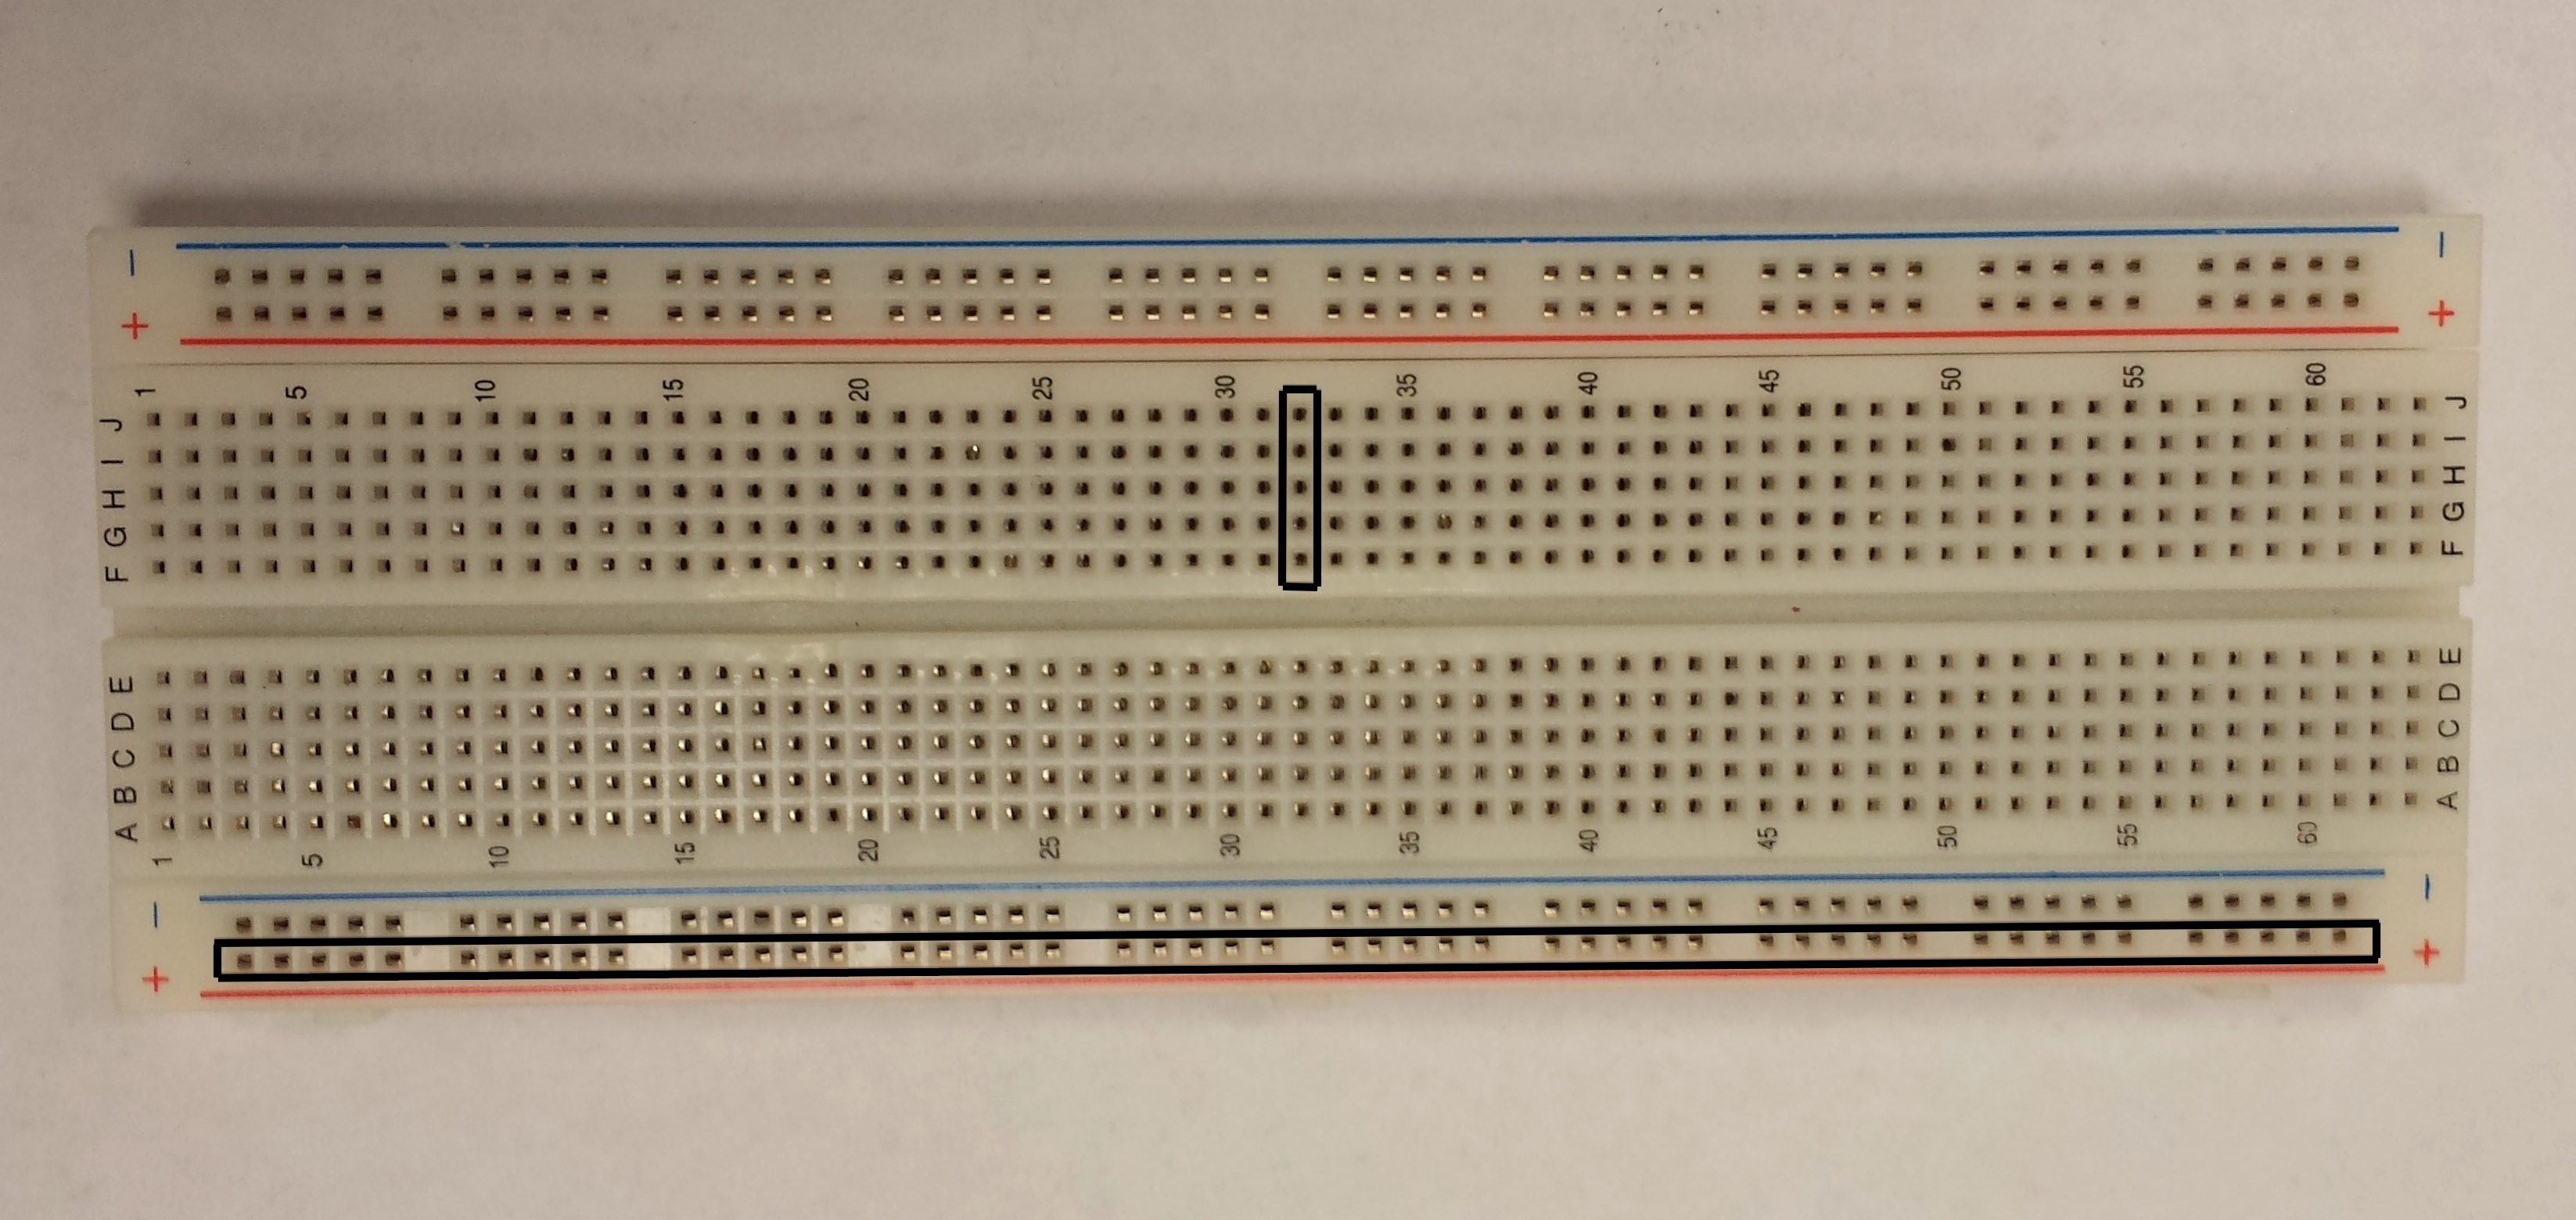
\includegraphics[width=\textwidth]{Images/physical_protoboard.jpg}
\caption{Physical protoboard. In the top and bottom groups, the dots are
interconnected horizontally. In the middle two groups, the dots are
interconnected vertically.}
\label{fig:physical_protoboard}
\end{center}
\end{figure}

\subsection{What is a protoboard layout of a circuit schematic?}

The protoboard layout of a given schematic is the placement of circuit pieces
and wires on a protoboard that corresponds to the schematic. This is done by
placing the appropriate pieces on the protoboard and then appropriately
interconnecting them with wires as prescribed by the schematic. As an example,
Figure \ref{fig:eg_s_to_pb} presents the protoboard layout corresponding to the
example schematic shown in Figure \ref{fig:schematic}.

\begin{figure}
\begin{center}
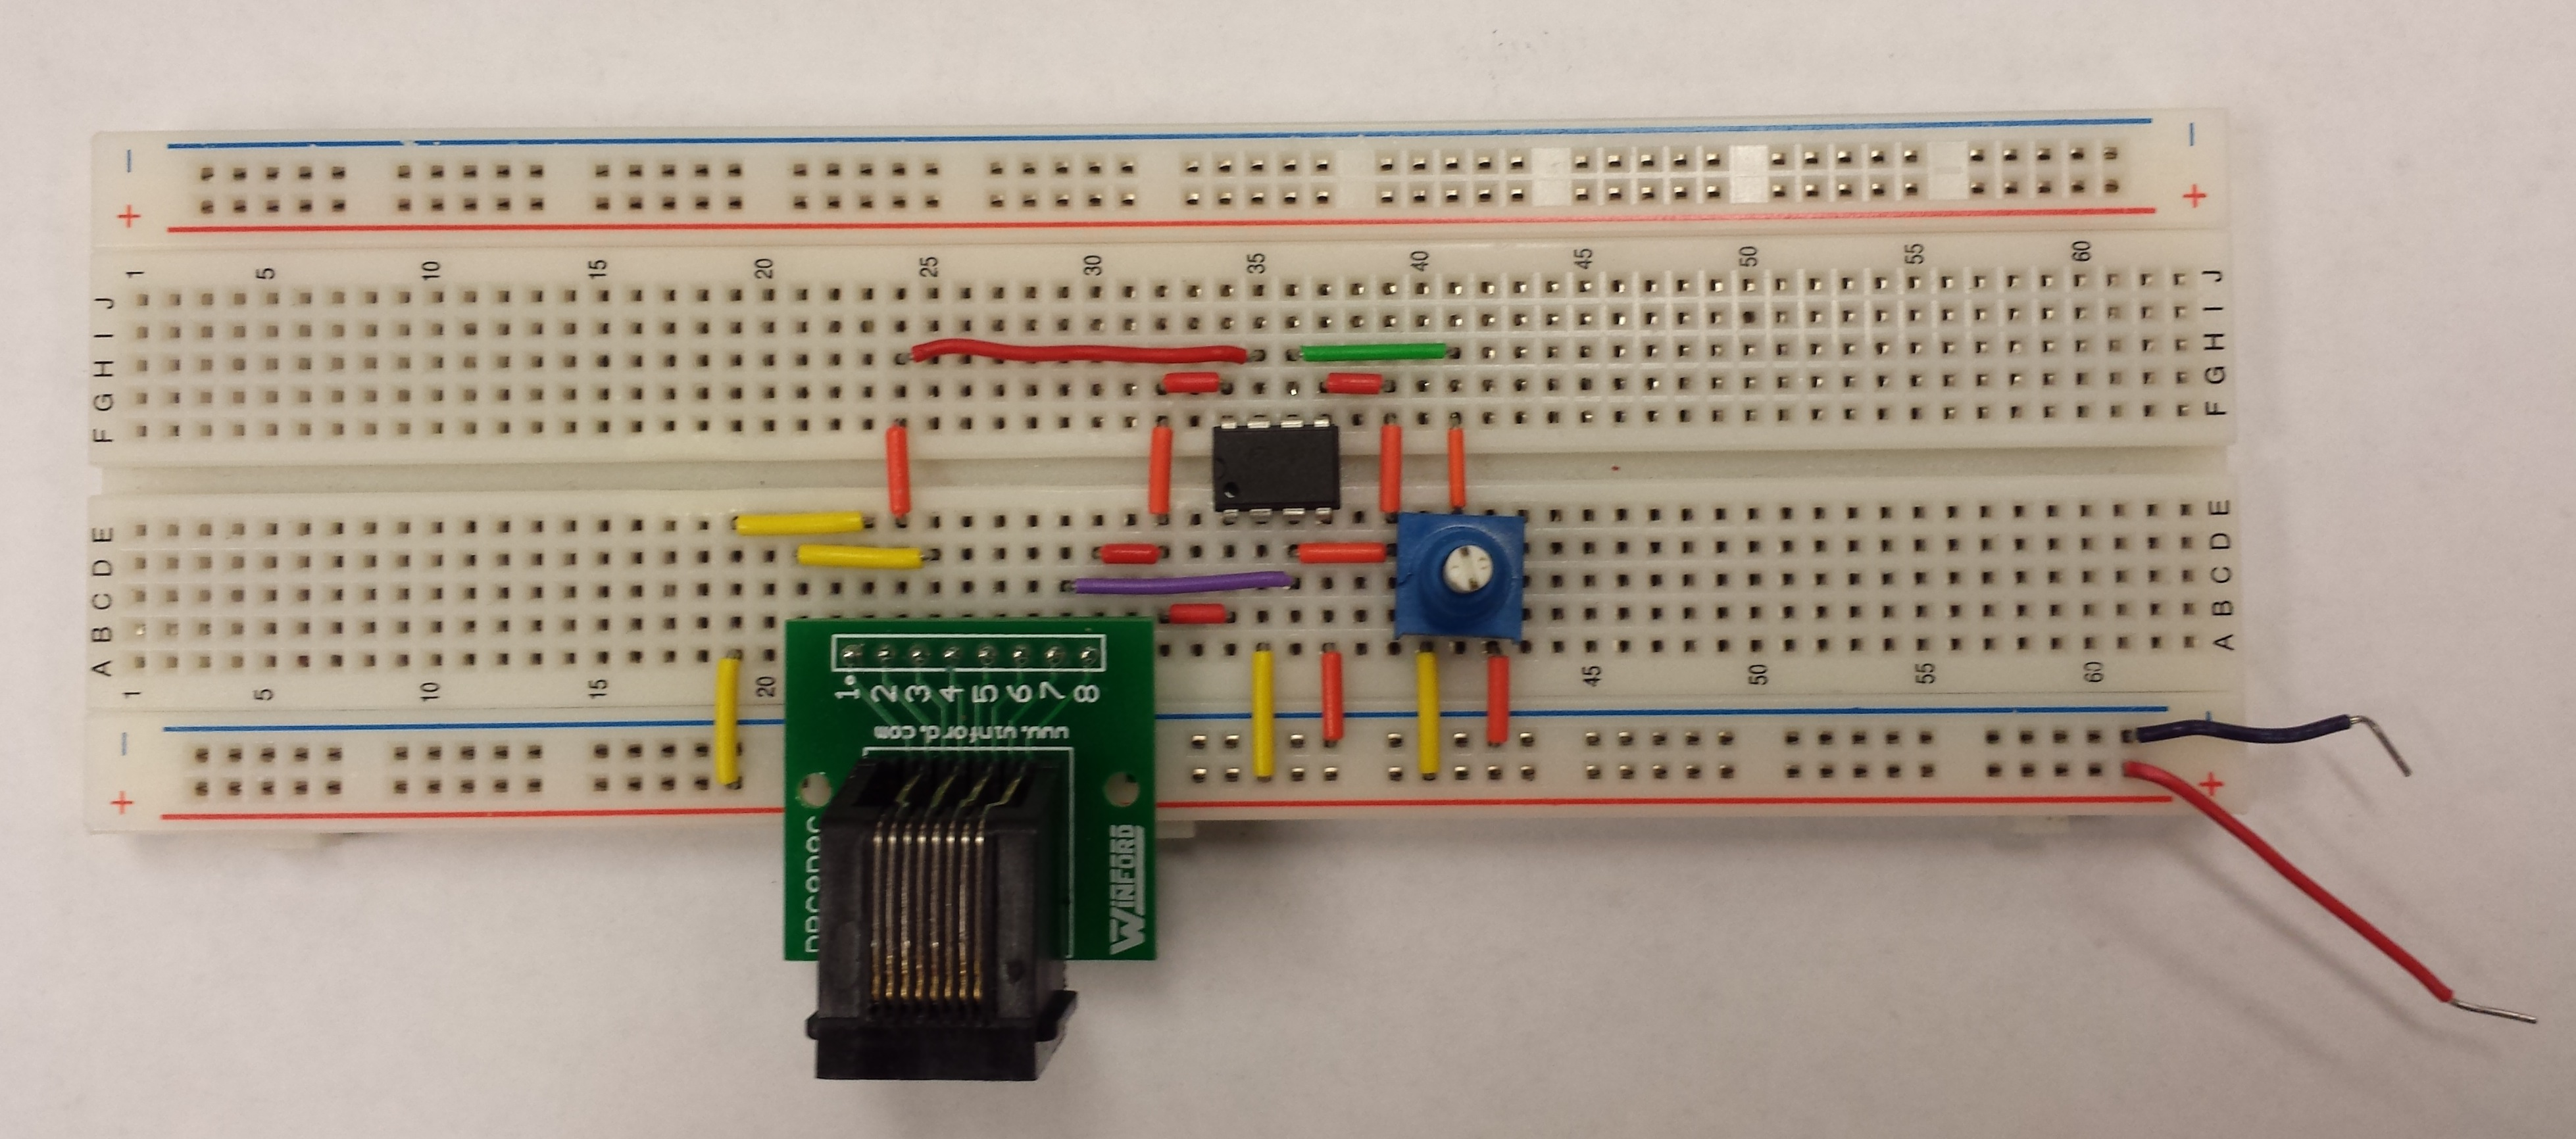
\includegraphics[width=\textwidth]{Images/sample_physical_layout.jpg}
\caption{Protoboard layout for the schematic in Figure \ref{fig:schematic}.}
\label{fig:eg_s_to_pb}
\end{center}
\end{figure}

For each of the circuit components we are interested in, there is a corresponding
circuit piece that may be inserted into the protoboard. The one exception is that
op-amps come in pairs. That is, each op-amp circuit piece that is inserted in the
protoboard actually contains two op-amp components within it. This raises an
important design question when we layout a schematic: what is the best way to
group together the op-amps in a schematic to result in the ``best'' layout? In
answering this question, the designer must have some criteria for what makes a
layout ``good.'' While there are no conclusive answers for this question,
general rules of thumb are (in no particular order):

\begin{itemize}
\item The layout should not have any wires that cross circuit pieces.
\item The layout should have no occlusions (i.e. crossing wires with identical
orientations).
\item The layout should have no crossing wires.
\item The layout should only have horizontal and vertical wires (i.e. no
diagonal wires).
\item The layout should have as few wires as possible.
\item The total length of wires in the layout should be as small as possible.
\end{itemize}

Given the background information discussed thus far, the goal of our project is
generating a ``good'' protoboard layout from circuit schematics automatically.

\section{Previous Work}

Here we will discuss previous work that has been done relating to this project.
First, as our project aims to augment the quality of 6.01, we look at the
current infrastructure available for students. Next, we look at what work has
been done relating to layout in general.

\subsection{CMax}

In a typical circuits lab in 6.01, students first design a circuit by drawing a
schematic of the circuit on paper and discussing their design with a staff
member. After they iteratively amend their design and are happy with it, they
build the circuit on a simulation tool called Circuits Maximus (CMax)\cite{cmax}.
With this
tool, students can layout their circuits on a simulated protoboard as if they
were laying it out on a physical one. CMax allows students to simulate the circuit
to make sure that it behaves as desired. Circuit layout is much easier on CMax
than on a physical protoboard. Hence, CMax provides a very fast and safe way of
debugging circuit layouts. Once the students are satisfied with their
observations from CMax, they build their circuits on physical protoboards and
carryout the appropriate experiments. Figure \ref{fig:cmax_sample} presents a
CMax layout of the schematic in Figure \ref{fig:schematic}.

\begin{figure}
\begin{center}
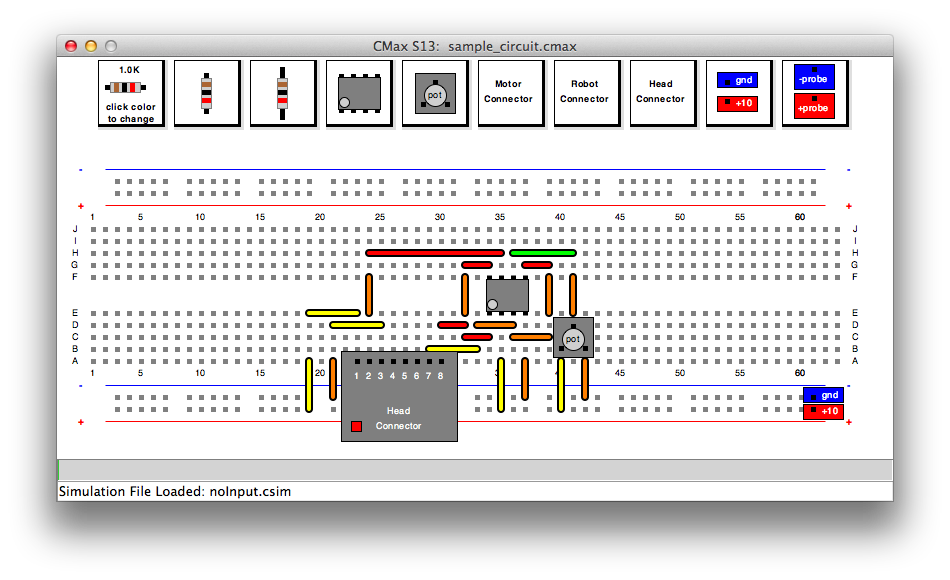
\includegraphics[width=\textwidth]{Images/sample_circuit.png}
\caption{CMax layout for the schematic in Figure \ref{fig:schematic}.}
\label{fig:cmax_sample}
\end{center}
\end{figure}

CMax has been a fantastic resource for 6.01 students. Its introduction has made
learning circuits significantly easier for many students, especially those that
have little or no prior experience with circuits. In addition to making the lab
exercises much more manageable, it provides students with a very handy way to
build, analyze, and experiment with circuits at their own leisure outside of lab.

While CMax is a fantastic tool, we can imagine a tool that can be even more
useful. The most instructive part of the labs that students do in the circuits
module of 6.01 is really designing the circuits in the first place, which they
currently do by drawing schematic diagrams on paper. Once they are happy with
their schematic diagrams, they proceed to laying out the corresponding circuits
with CMax. The process of laying out a schematic does not really have very much
instructive substance. This process is essentially solving a puzzle, and has
almost nothing to do with the subject matter -- designing circuits. In fact,
when the circuits get complicated and involve many pieces, translating a
schematic diagram into a protoboard layout gets to be quite challenging and
time-consuming. In these situations, students often end up with convoluted and
unpleasant layouts that are very difficult to debug in the likely case of the
circuit not behaving as expected. Not only are such layouts difficult to debug
for the students themselves, but they are also often difficult for staff
members to fathom.

In the best case scenario, students should not have to produce protoboard
layouts for their schematic diagrams. Indeed they should work out the right
schematic diagram of the circuit of interest, but the layout generation should
not be part of the learning process. This project aims to let students draw and
analyze schematic drawings of circuits and produce the corresponding protoboard
layouts automatically. Given the protoboard layouts output by this tool,
students can proceed to building the circuits on physical protoboards and
carrying out the appropriate experiments.

With this tool, a typical circuits lab would go as follows. First, as before,
the students draw schematic diagrams of their circuits on paper. Once they have
schematic drawings they are happy with, they can directly draw their schematic
drawings on the simulation tool. In fact, students my go straight to building
the schematic drawings on the simulation tool, bypassing the experimentation on
paper. Once they have a schematic drawn, they can analyze it with the tool,
discuss it with staff members, and amend it easily and quickly with the
user-friendly GUI of the simulation tool. When they are
satisfied with the behaviors of their schematic circuit, they can produce the
corresponding protoboard layout simply at the click of a button -- this would be
the most important advantage of this tool. They can then build the layout on a
physical protoboard and carryout experiments with it.

\subsection{Current work in automatic layout}

In my explorations, I was not able to find any tools that completely
automatically convert circuit schematics into protoboard layouts. However, there
do exists tools that perform partially- or fully-automatic Printed Circuit
Board (PCB) layout. To my findings, most of these tools do not publish their
algorithms and, rather, keep them proprietary. Hence, I was not able to build my
work off of any existing products. In a sense, this project aims to build
something new.
